%
% Sección de funciones hash, capítulo de antecedentes.
% Proyecto Lovelace.
%

\section{Funciones hash}
\label{sec:hash}

La información presentada a continuación puede consultarse con más profundidad
en las siguientes referencias
\cite{hash_hussein, menezes, DBLP:series/isc/DelfsK07, hash_gupta}.

Se refiere al conjunto de funciones computacionalmente eficientes que
mapean cadenas binarias de una longitud arbitraria a cadenas binarias
de una longitud fija, llamadas valores hash.

\begin{figure}
  \begin{center}
    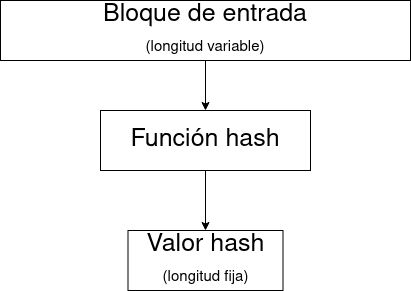
\includegraphics[width=0.6\linewidth]{diagramas/hash}
    \caption{Diagrama del funcionamiento de una función hash.}
   \end{center}
\end{figure}


Matemáticamente, una función hash es una función
\begin{equation}
  \label{funcion_hash_def}
  \begin{split}
    h: \{0, 1\}^* \longrightarrow \{0,1\}^n \\
    m \longmapsto h(m)
  \end{split}
\end{equation}
La longitud de $n$ suele ser entre 128 y 512 bits. Las funciones hash
$h$ tienen las siguientes propiedades:

\begin{enumerate}
  \item Compresión: $h$ mapea una entrada $x$ (cuya longitud
    finita es arbitraria) a una salida $h(x)$ de longitud fija $n$.
  \item Facilidad de cómputo: dada $x$ y $h$, $h(x)$ es
    calculada ya sea sin necesitar mucho espacio, tiempo de cómputo, o
    requiere pocas operaciones, etcétera.
\end{enumerate}

De manera general, las funciones hash se pueden dividir en dos
categorías: las que no utilizan llave y su único parámetro es la entrada
$x$, y las que necesitan una llave secreta $k$ y la entrada $x$.

Sea una función hash sin llave $h$ con entradas $x$, $x^\prime$ y
salidas $y$ y $y^\prime$, respectivamente. A continuación se listan
algunas de las propiedades que puede tener:

\begin{enumerate}
  \item Resistencia de \gls{gl:preimagen}: no es computacionalmente factible
    para una salida específica $y$ encontrar una entrada $x^\prime$ que
    dé como resultado el mismo valor hash $h(x^\prime) = y$ si no se
    conoce $x$. Esta propiedad también es llamada
    \textit{de un sentido}.
  \item Resistencia de segunda \gls{gl:preimagen}: no es computacionalmente
    factible encontrar una segunda entrada $x^\prime$  que tenga la
    misma salida que una entrada específica $x$: $x \neq x^\prime$
    tal que $h(x) = h(x^\prime)$. Esta propiedad también es conocida
    como \textit{de débil resistencia a colisiones}.
  \item Resistencia a las colisiones: no es computacionalmente factible
    encontrar dos entradas distintas $x$, $x^\prime$ que lleven al
    mismo valor hash, o sea, $h(x) = h(x^\prime)$. A diferencia de la
    anterior, la selección de ambas entradas no está restringida. Esta
    propiedad también es conocida como
    \textit{de gran resistencia a colisiones}.
\end{enumerate}

Una función hash $h$ que cumple con las propiedades de resistencia de
\gls{gl:preimagen} y resistencia de segunda \gls{gl:preimagen} es conocida como
una función hash de un solo sentido o \gls{gl:owhf}.
Las que cumplen con la resistencia de segunda \gls{gl:preimagen} y
resistencia a las colisiones son conocidas como funciones hash
resistentes a colisiones o \gls{gl:crhf}. Aunque casi siempre las
funciones \gls{gl:crhf} cumplen con la resistencia de \gls{gl:preimagen},
no es obligatorio que lo hagan.

Algunos ejemplos de las funciones \gls{gl:owhf} son el \gls{gl:sha}-1
y el \gls{gl:md5}. En los esquemas de firma electrónica, se obtiene el
valor hash del mensaje ($h(m)$) y se pone en el lugar de la firma. Los valores
hash también son utilizados para revisar la integridad de las llaves
públicas y, al utilizarse con una llave secreta, las funciones
criptográficas hash se convierten en códigos de autenticación de mensaje
(\gls{gl:mac}, por sus siglas en inglés), una de las herramientas más
utilizadas en protocolos como \gls{gl:ssl} e IPSec para revisar la
integridad de un mensaje y autenticar al remitente.

Una de las aplicaciones más conocidas de las funciones hash es la de
cifrar las contraseñas: en un sistema, en vez de almacenar la contraseña
$clave$, se guarda su valor hash $h(clave)$. Así, cuando un usuario
ingresa su contraseña, el sistema calcula su valor hash y lo compara con
el que se tiene guardado. Realizar esto ayuda a evitar que las
contraseñas sean conocidas para los usuarios con privilegios, como
pueden ser los administradores.

\subsection{Integridad de datos}

Las funciones criptográficas hash también son conocidas como funciones
\textit{procesadoras de mensajes} y el valor hash $h(m)$ de un mensaje
$m$ dado es llamado \textit{huella} de $m$; ya que es una representación
compacta de m y, dada la resistencia a la segunda \gls{gl:preimagen}, la huella
es prácticamente única. Si el mensaje fuese modificado, el valor hash
sería distinto; por lo que si se tienen almacenados los valores hash,
basta con calcular su valor $h(m)$ y compararlo con el que se tiene
guardado para detectar modificaciones. Por esta razón, las funciones
hash también son llamadas códigos de detección de modificaciones (como el
\gls{gl:mdc2}).

\subsection{Firmas}

Sea $(n, e)$ la llave pública \gls{gl:rsa} y $d$ el exponente decodificador
secreto de Alice. En el esquema básico de firma \gls{gl:rsa}, Alice puede
firmar mensajes que estén codificados por números $ m \in \{0, \dots, n-1\}$.
Para firmar $m$, aplica el algoritmo de descifrado y obtiene la firma
$\sigma = m^d$ $mod$ $n$ de $m$.
Normalmente, $n$ es un número de 1024 bits y Alice puede firmar una
cadena de bits $m$ tal que, cuando es interpretada como número, sea
menor que $n$. Esto es una cadena de, máximo, 128 caracteres
\gls{gl:ascii}: la mayoría de los documentos que se desean firmar suelen
ser mucho más grandes. Este problema existe en todos los esquemas de firma
digital y usualmente es resuelto al aplicar una función hash resistente a
colisiones $h$. De esta forma, primero se obtiene el valor hash del mensaje
$h(m)$ y esto es lo que se firma en lugar del mensaje mismo ($m$):
\begin{equation}
  \label{funcion_hash_sign}
  \sigma = h(m)^d \quad mod \quad n
\end{equation}

Los mensajes que tengan el mismo valor hash tienen la misma firma. En
este caso, es primordial que la función hash $h$ sea resistente a
colisiones para garantizar el no repudio. De otra manera, Alice podría
firmar el mensaje $m$ y después decir que había firmado un mensaje
distinto ($n$).
La resistencia a segundas preimágenes previene que un atacante Eve tome
un mensaje $m$ firmado por Alice, genere un mensaje nuevo $n$ y utilice
$\sigma$ como una firma válida de Alice para $n$.

\subsection{Message Digest-4 (MD4)}

En la década de 1990 esta función hash fue diseñada por Ronald Rivest.
Tiene entradas de longitud arbitraria y la longitud de la salida
procesada es de 128 bits. El \gls{gl:md4} fue innovador y
clave en el diseño para los algoritmos venideros de esta clase (como
el \gls{gl:md5}).

\subsection{RIPEMD}

Esta función hash, publicada en 1996, está basada en \gls{gl:md4} y fue
diseñada por Hans Dobbertin y otros. Consiste en dos formas equivalentes de la
función de compresión de \gls{gl:md4}. El algoritmo original (RIPEMD-160)
devuelve bloques \textit{procesados} de 160 bits; cuando en 1996 Hans
descubrió una colisión en dos rondas, se desarrollaron nuevas versiones
mejoradas: RIPEMD-128, RIPE-256, RIPE-320; las cuales dan bloques procesados de
128, 256 y 320 bits respectivamente.

\subsection{\textit{Secure Hash Algorithm (SHA)}}

El algoritmo \gls{gl:sha} fue publicado por \gls{gl:nist} y
\gls{gl:nsa} en 1993; este algoritmo produce bloques de 160 bits y
fue desarrollado para reemplazar al \gls{gl:md4}; sin embargo, poco
después de haber sido publicado tuvo que ser quitado por problemas de
seguridad. Actualmente, \gls{gl:sha} es conocido como \gls{gl:sha}-0.

En 1995, \gls{gl:sha}-0 fue reemplazado por \gls{gl:sha}-1; tiene
una salida de la misma longitud que su predecesor y es una de las funciones
hash más populares. Hay que destacar que la seguridad que brinda esta función
es limitada, pues tiene el mismo nivel que un cifrado por bloques de 80 bits.

En 2002 \gls{gl:nist} publicó tres funciones hash más:
\gls{gl:sha}-256, \gls{gl:sha}-384 y \gls{gl:sha}-512; esta
familia de funciones hash es conocida como \gls{gl:sha}-2 y fue
desarrollada para cubrir la necesidad de una llave más grande para poder
empatar su tamaño con \gls{gl:aes}. Dos años más tarde, una nueva
función hash fue agregada a la familia \gls{gl:sha}-2:
\gls{gl:sha}-224.

Finalmente, en 2008, \gls{gl:nist} inició un concurso para buscar al
\gls{gl:sha}-3 y en 2012 anunció al ganador: Keccak, una función hash
desarrollada por Guido Bertoni, Joan Daemen, Michael Peeters y Gilles Van
Assche. Esta función tiene una construcción completamente distinta a las
familias anteriores.
